\newcommand{\coursemodule}{Module 03}
% ════════════════════════════════════════════════════════════════════════════
% Pixels, Frames & Transformers: shared Beamer preamble (WUR style)
% Adapted from the preamble of Bags, Vectors & Transformers.
%
% Use in a module deck (from <part>/<module>/slides/):
%   \newcommand{\coursemodule}{Module 01}
%   % ════════════════════════════════════════════════════════════════════════════
% Pixels, Frames & Transformers: shared Beamer preamble (WUR style)
% Adapted from the preamble of Bags, Vectors & Transformers.
%
% Use in a module deck (from <part>/<module>/slides/):
%   \newcommand{\coursemodule}{Module 01}
%   % ════════════════════════════════════════════════════════════════════════════
% Pixels, Frames & Transformers: shared Beamer preamble (WUR style)
% Adapted from the preamble of Bags, Vectors & Transformers.
%
% Use in a module deck (from <part>/<module>/slides/):
%   \newcommand{\coursemodule}{Module 01}
%   \input{../../../shared/preamble.tex}
%   \begin{document}
%   \moduletitle{Images as Data}
%   ...
% Compile with: latexmk -pdf <deck>.tex
% ════════════════════════════════════════════════════════════════════════════

\documentclass[aspectratio=169]{beamer}

% ── Packages ────────────────────────────────────────────────────────────────
\usepackage[T1]{fontenc}
\usepackage[utf8]{inputenc}
\usepackage{lmodern}
\usepackage{microtype}
\usepackage{xcolor}
\usepackage{tikz}
\usetikzlibrary{arrows.meta, positioning, calc, shapes.geometric, decorations.pathreplacing, matrix, fit}
\usepackage{booktabs}
\usepackage{fontawesome5}
\usepackage{array}
\usepackage[most]{tcolorbox}

\providecommand{\coursemodule}{}

% ── WUR color palette ───────────────────────────────────────────────────────
\definecolor{wurgreen}{HTML}{34B233}
\definecolor{darkgreen}{HTML}{1F6B1E}
\definecolor{lightgreen}{HTML}{E8F7E8}
\definecolor{darknavy}{HTML}{1A1A2E}
\definecolor{midgray}{HTML}{6B7280}
\definecolor{lightgray}{HTML}{F3F4F6}
\definecolor{bodytext}{HTML}{1F2937}
\definecolor{codegreen}{HTML}{9AE6B4}
\definecolor{warnred}{HTML}{FEE2E2}
\definecolor{warnborder}{HTML}{EF4444}

% ── Beamer theme ────────────────────────────────────────────────────────────
\usetheme{default}
\usecolortheme{default}
\usefonttheme{professionalfonts}
\setbeamertemplate{navigation symbols}{}
\setbeamertemplate{itemize items}{\textcolor{wurgreen}{\textbullet}}
\setbeamertemplate{itemize subitem}{\textcolor{midgray}{--}}
\setbeamertemplate{enumerate items}{\textcolor{wurgreen}{\textbf{\insertenumlabel.}}}
\setbeamercolor{frametitle}{fg=white, bg=darknavy}
\setbeamertemplate{frametitle}{%
  \begin{beamercolorbox}[wd=\paperwidth, ht=1.1cm, dp=0.2cm, leftskip=0.6cm]{frametitle}
    \usebeamerfont{frametitle}\insertframetitle
  \end{beamercolorbox}%
}
\setbeamerfont{frametitle}{size=\large, series=\bfseries}
\setbeamercolor{background canvas}{bg=white}
\setbeamercolor{normal text}{fg=bodytext}
\setbeamerfont{normal text}{size=\small}
\setbeamertemplate{footline}{%
  \begin{beamercolorbox}[wd=\paperwidth, ht=0.4cm, dp=0.15cm]{footline}%
    \hspace{0.5cm}%
    \textcolor{midgray}{\tiny Pixels, Frames \& Transformers · \coursemodule\ · Wageningen University \& Research}%
    \hfill%
    \textcolor{midgray}{\tiny \insertframenumber}%
    \hspace{0.4cm}%
  \end{beamercolorbox}%
}

% ── Boxes ───────────────────────────────────────────────────────────────────
\tcbset{wurbase/.style={arc=3pt, boxrule=0.6pt, left=7pt, right=7pt, top=5pt, bottom=5pt,
                        fontupper=\small, before skip=4pt, after skip=4pt}}
\newtcolorbox{greenbox}[1][]{wurbase, colback=lightgreen, colframe=wurgreen, #1}
\newtcolorbox{graybox}[1][]{wurbase, colback=lightgray, colframe=lightgray, #1}
\newtcolorbox{navybox}[1][]{wurbase, colback=darknavy, colframe=darknavy, colupper=white, #1}
\newtcolorbox{warnbox}[1][]{wurbase, colback=warnred, colframe=warnborder, #1}
\newtcolorbox{codebox}[1][]{wurbase, colback=darknavy, colframe=darknavy, colupper=white,
                            fontupper=\ttfamily\scriptsize, left=6pt, top=4pt, bottom=4pt, #1}

% ── Title slide ─────────────────────────────────────────────────────────────
\newcommand{\moduletitle}[1]{%
{
\setbeamertemplate{footline}{}
\begin{frame}[plain]
  \begin{tikzpicture}[remember picture, overlay]
    \fill[darknavy] (current page.south west) rectangle (current page.north east);
    \fill[wurgreen] (current page.south west) rectangle ([xshift=0.45cm]current page.north west);
    \node[anchor=west, text=white, font=\huge\bfseries, text width=13cm]
      at ([xshift=1.1cm, yshift=1.2cm]current page.west) {Pixels, Frames \& Transformers};
    \node[anchor=west, text=wurgreen, font=\large, text width=13cm]
      at ([xshift=1.1cm, yshift=0.05cm]current page.west) {#1 · \coursemodule};
    \node[anchor=west, text=midgray, font=\small, text width=12cm]
      at ([xshift=1.1cm, yshift=-1.5cm]current page.west)
      {Denise J. Roth, PhD Candidate\\
       Strategic Communication Group · Wageningen University \& Research};
  \end{tikzpicture}
\end{frame}
}}

% ── Small helpers ───────────────────────────────────────────────────────────
\newcommand{\keyterm}[1]{\textbf{\textcolor{darkgreen}{#1}}}
\newcommand{\muted}[1]{\textcolor{midgray}{#1}}
\newcommand{\credit}[1]{{\tiny\textcolor{midgray}{#1}}}
\newcommand{\notebookslide}[1]{%
\begin{frame}{In the Notebook}
\vspace{0.1cm}
#1
\end{frame}}
\newcommand{\nbitem}[2]{\item[\textcolor{wurgreen}{#1}] #2}

%   \begin{document}
%   \moduletitle{Images as Data}
%   ...
% Compile with: latexmk -pdf <deck>.tex
% ════════════════════════════════════════════════════════════════════════════

\documentclass[aspectratio=169]{beamer}

% ── Packages ────────────────────────────────────────────────────────────────
\usepackage[T1]{fontenc}
\usepackage[utf8]{inputenc}
\usepackage{lmodern}
\usepackage{microtype}
\usepackage{xcolor}
\usepackage{tikz}
\usetikzlibrary{arrows.meta, positioning, calc, shapes.geometric, decorations.pathreplacing, matrix, fit}
\usepackage{booktabs}
\usepackage{fontawesome5}
\usepackage{array}
\usepackage[most]{tcolorbox}

\providecommand{\coursemodule}{}

% ── WUR color palette ───────────────────────────────────────────────────────
\definecolor{wurgreen}{HTML}{34B233}
\definecolor{darkgreen}{HTML}{1F6B1E}
\definecolor{lightgreen}{HTML}{E8F7E8}
\definecolor{darknavy}{HTML}{1A1A2E}
\definecolor{midgray}{HTML}{6B7280}
\definecolor{lightgray}{HTML}{F3F4F6}
\definecolor{bodytext}{HTML}{1F2937}
\definecolor{codegreen}{HTML}{9AE6B4}
\definecolor{warnred}{HTML}{FEE2E2}
\definecolor{warnborder}{HTML}{EF4444}

% ── Beamer theme ────────────────────────────────────────────────────────────
\usetheme{default}
\usecolortheme{default}
\usefonttheme{professionalfonts}
\setbeamertemplate{navigation symbols}{}
\setbeamertemplate{itemize items}{\textcolor{wurgreen}{\textbullet}}
\setbeamertemplate{itemize subitem}{\textcolor{midgray}{--}}
\setbeamertemplate{enumerate items}{\textcolor{wurgreen}{\textbf{\insertenumlabel.}}}
\setbeamercolor{frametitle}{fg=white, bg=darknavy}
\setbeamertemplate{frametitle}{%
  \begin{beamercolorbox}[wd=\paperwidth, ht=1.1cm, dp=0.2cm, leftskip=0.6cm]{frametitle}
    \usebeamerfont{frametitle}\insertframetitle
  \end{beamercolorbox}%
}
\setbeamerfont{frametitle}{size=\large, series=\bfseries}
\setbeamercolor{background canvas}{bg=white}
\setbeamercolor{normal text}{fg=bodytext}
\setbeamerfont{normal text}{size=\small}
\setbeamertemplate{footline}{%
  \begin{beamercolorbox}[wd=\paperwidth, ht=0.4cm, dp=0.15cm]{footline}%
    \hspace{0.5cm}%
    \textcolor{midgray}{\tiny Pixels, Frames \& Transformers · \coursemodule\ · Wageningen University \& Research}%
    \hfill%
    \textcolor{midgray}{\tiny \insertframenumber}%
    \hspace{0.4cm}%
  \end{beamercolorbox}%
}

% ── Boxes ───────────────────────────────────────────────────────────────────
\tcbset{wurbase/.style={arc=3pt, boxrule=0.6pt, left=7pt, right=7pt, top=5pt, bottom=5pt,
                        fontupper=\small, before skip=4pt, after skip=4pt}}
\newtcolorbox{greenbox}[1][]{wurbase, colback=lightgreen, colframe=wurgreen, #1}
\newtcolorbox{graybox}[1][]{wurbase, colback=lightgray, colframe=lightgray, #1}
\newtcolorbox{navybox}[1][]{wurbase, colback=darknavy, colframe=darknavy, colupper=white, #1}
\newtcolorbox{warnbox}[1][]{wurbase, colback=warnred, colframe=warnborder, #1}
\newtcolorbox{codebox}[1][]{wurbase, colback=darknavy, colframe=darknavy, colupper=white,
                            fontupper=\ttfamily\scriptsize, left=6pt, top=4pt, bottom=4pt, #1}

% ── Title slide ─────────────────────────────────────────────────────────────
\newcommand{\moduletitle}[1]{%
{
\setbeamertemplate{footline}{}
\begin{frame}[plain]
  \begin{tikzpicture}[remember picture, overlay]
    \fill[darknavy] (current page.south west) rectangle (current page.north east);
    \fill[wurgreen] (current page.south west) rectangle ([xshift=0.45cm]current page.north west);
    \node[anchor=west, text=white, font=\huge\bfseries, text width=13cm]
      at ([xshift=1.1cm, yshift=1.2cm]current page.west) {Pixels, Frames \& Transformers};
    \node[anchor=west, text=wurgreen, font=\large, text width=13cm]
      at ([xshift=1.1cm, yshift=0.05cm]current page.west) {#1 · \coursemodule};
    \node[anchor=west, text=midgray, font=\small, text width=12cm]
      at ([xshift=1.1cm, yshift=-1.5cm]current page.west)
      {Denise J. Roth, PhD Candidate\\
       Strategic Communication Group · Wageningen University \& Research};
  \end{tikzpicture}
\end{frame}
}}

% ── Small helpers ───────────────────────────────────────────────────────────
\newcommand{\keyterm}[1]{\textbf{\textcolor{darkgreen}{#1}}}
\newcommand{\muted}[1]{\textcolor{midgray}{#1}}
\newcommand{\credit}[1]{{\tiny\textcolor{midgray}{#1}}}
\newcommand{\notebookslide}[1]{%
\begin{frame}{In the Notebook}
\vspace{0.1cm}
#1
\end{frame}}
\newcommand{\nbitem}[2]{\item[\textcolor{wurgreen}{#1}] #2}

%   \begin{document}
%   \moduletitle{Images as Data}
%   ...
% Compile with: latexmk -pdf <deck>.tex
% ════════════════════════════════════════════════════════════════════════════

\documentclass[aspectratio=169]{beamer}

% ── Packages ────────────────────────────────────────────────────────────────
\usepackage[T1]{fontenc}
\usepackage[utf8]{inputenc}
\usepackage{lmodern}
\usepackage{microtype}
\usepackage{xcolor}
\usepackage{tikz}
\usetikzlibrary{arrows.meta, positioning, calc, shapes.geometric, decorations.pathreplacing, matrix, fit}
\usepackage{booktabs}
\usepackage{fontawesome5}
\usepackage{array}
\usepackage[most]{tcolorbox}

\providecommand{\coursemodule}{}

% ── WUR color palette ───────────────────────────────────────────────────────
\definecolor{wurgreen}{HTML}{34B233}
\definecolor{darkgreen}{HTML}{1F6B1E}
\definecolor{lightgreen}{HTML}{E8F7E8}
\definecolor{darknavy}{HTML}{1A1A2E}
\definecolor{midgray}{HTML}{6B7280}
\definecolor{lightgray}{HTML}{F3F4F6}
\definecolor{bodytext}{HTML}{1F2937}
\definecolor{codegreen}{HTML}{9AE6B4}
\definecolor{warnred}{HTML}{FEE2E2}
\definecolor{warnborder}{HTML}{EF4444}

% ── Beamer theme ────────────────────────────────────────────────────────────
\usetheme{default}
\usecolortheme{default}
\usefonttheme{professionalfonts}
\setbeamertemplate{navigation symbols}{}
\setbeamertemplate{itemize items}{\textcolor{wurgreen}{\textbullet}}
\setbeamertemplate{itemize subitem}{\textcolor{midgray}{--}}
\setbeamertemplate{enumerate items}{\textcolor{wurgreen}{\textbf{\insertenumlabel.}}}
\setbeamercolor{frametitle}{fg=white, bg=darknavy}
\setbeamertemplate{frametitle}{%
  \begin{beamercolorbox}[wd=\paperwidth, ht=1.1cm, dp=0.2cm, leftskip=0.6cm]{frametitle}
    \usebeamerfont{frametitle}\insertframetitle
  \end{beamercolorbox}%
}
\setbeamerfont{frametitle}{size=\large, series=\bfseries}
\setbeamercolor{background canvas}{bg=white}
\setbeamercolor{normal text}{fg=bodytext}
\setbeamerfont{normal text}{size=\small}
\setbeamertemplate{footline}{%
  \begin{beamercolorbox}[wd=\paperwidth, ht=0.4cm, dp=0.15cm]{footline}%
    \hspace{0.5cm}%
    \textcolor{midgray}{\tiny Pixels, Frames \& Transformers · \coursemodule\ · Wageningen University \& Research}%
    \hfill%
    \textcolor{midgray}{\tiny \insertframenumber}%
    \hspace{0.4cm}%
  \end{beamercolorbox}%
}

% ── Boxes ───────────────────────────────────────────────────────────────────
\tcbset{wurbase/.style={arc=3pt, boxrule=0.6pt, left=7pt, right=7pt, top=5pt, bottom=5pt,
                        fontupper=\small, before skip=4pt, after skip=4pt}}
\newtcolorbox{greenbox}[1][]{wurbase, colback=lightgreen, colframe=wurgreen, #1}
\newtcolorbox{graybox}[1][]{wurbase, colback=lightgray, colframe=lightgray, #1}
\newtcolorbox{navybox}[1][]{wurbase, colback=darknavy, colframe=darknavy, colupper=white, #1}
\newtcolorbox{warnbox}[1][]{wurbase, colback=warnred, colframe=warnborder, #1}
\newtcolorbox{codebox}[1][]{wurbase, colback=darknavy, colframe=darknavy, colupper=white,
                            fontupper=\ttfamily\scriptsize, left=6pt, top=4pt, bottom=4pt, #1}

% ── Title slide ─────────────────────────────────────────────────────────────
\newcommand{\moduletitle}[1]{%
{
\setbeamertemplate{footline}{}
\begin{frame}[plain]
  \begin{tikzpicture}[remember picture, overlay]
    \fill[darknavy] (current page.south west) rectangle (current page.north east);
    \fill[wurgreen] (current page.south west) rectangle ([xshift=0.45cm]current page.north west);
    \node[anchor=west, text=white, font=\huge\bfseries, text width=13cm]
      at ([xshift=1.1cm, yshift=1.2cm]current page.west) {Pixels, Frames \& Transformers};
    \node[anchor=west, text=wurgreen, font=\large, text width=13cm]
      at ([xshift=1.1cm, yshift=0.05cm]current page.west) {#1 · \coursemodule};
    \node[anchor=west, text=midgray, font=\small, text width=12cm]
      at ([xshift=1.1cm, yshift=-1.5cm]current page.west)
      {Denise J. Roth, PhD Candidate\\
       Strategic Communication Group · Wageningen University \& Research};
  \end{tikzpicture}
\end{frame}
}}

% ── Small helpers ───────────────────────────────────────────────────────────
\newcommand{\keyterm}[1]{\textbf{\textcolor{darkgreen}{#1}}}
\newcommand{\muted}[1]{\textcolor{midgray}{#1}}
\newcommand{\credit}[1]{{\tiny\textcolor{midgray}{#1}}}
\newcommand{\notebookslide}[1]{%
\begin{frame}{In the Notebook}
\vspace{0.1cm}
#1
\end{frame}}
\newcommand{\nbitem}[2]{\item[\textcolor{wurgreen}{#1}] #2}


\begin{document}

\moduletitle{Handcrafted Features}

% ─────────────────────────────────────────────────────────────────────────────
\begin{frame}{Why Measure by Hand?}
Before deep learning, computer vision meant designing measurements by hand. In social science
they are often still the right tool:

\vspace{0.1cm}
\begin{columns}[T]
\begin{column}{0.31\textwidth}
\begin{greenbox}[height=2.3cm]
\textbf{\faFileImage\ Transparent}\\
You can write the formula in your methods section.
\end{greenbox}
\end{column}
\begin{column}{0.31\textwidth}
\begin{greenbox}[height=2.3cm]
\raggedright\textbf{\faMicrochip\ Cheap}\\
Seconds per thousand images on a laptop. No GPU needed.
\end{greenbox}
\end{column}
\begin{column}{0.31\textwidth}
\begin{greenbox}[height=2.3cm]
\raggedright\textbf{\faRuler\ Close to a construct}\\
Colorfulness, clutter, the size of a face: easy to link to theory.
\end{greenbox}
\end{column}
\end{columns}

\begin{warnbox}
\textbf{But a precise number is not automatically a valid measure.} Every feature here responds
to everything in the frame, so each needs a check against what you want to measure.
\end{warnbox}
\muted{The \texttt{athec} library collects dozens more such measures, with references (Peng, 2022).}
\end{frame}

% ─────────────────────────────────────────────────────────────────────────────
\begin{frame}{Light: Brightness and Contrast}
\begin{columns}[c]
\begin{column}{0.6\textwidth}
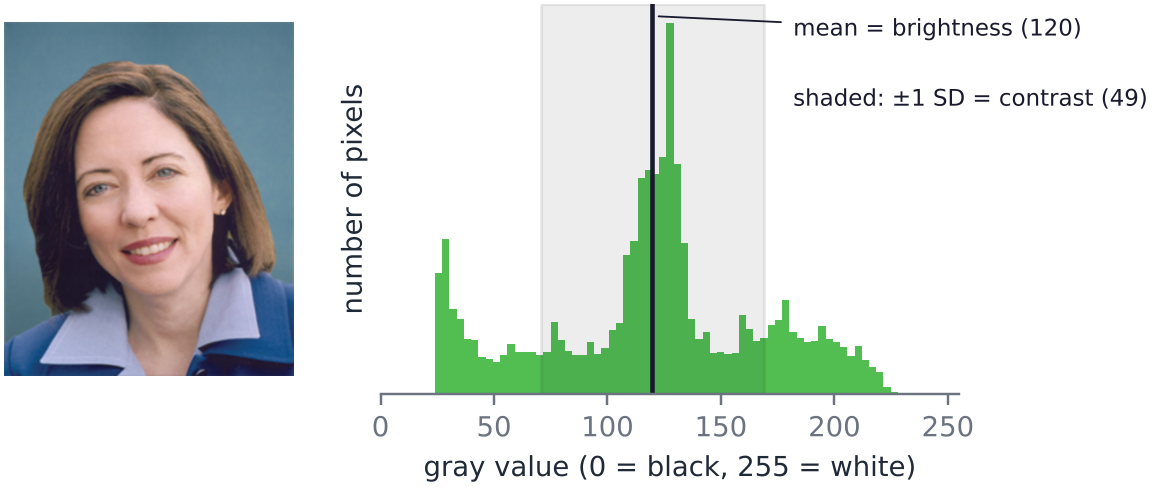
\includegraphics[width=\textwidth]{figures/light_histogram.png}
\end{column}
\begin{column}{0.37\textwidth}
\begin{itemize}
\item \keyterm{Brightness}: the mean gray value (0--255)
\item \keyterm{Contrast}: the standard deviation of the gray values
\item \keyterm{Clipped pixels}: the share almost black ($<$ 30) or almost white ($>$ 225)
\end{itemize}
\end{column}
\end{columns}

\vspace{0.2cm}
\begin{graybox}
On product photos, the brightest scores often come from a white background around the product,
not from the package itself. The whole frame is part of the measurement.
\end{graybox}
\vfill
\credit{Official portrait of Sen.\ Maria Cantwell, public domain, via unitedstates/images.}
\end{frame}

% ─────────────────────────────────────────────────────────────────────────────
\begin{frame}{Color: Saturation and Colorfulness}
\begin{columns}[T]
\begin{column}{0.38\textwidth}
\keyterm{Saturation}: the mean of the HSV saturation channel, how far colors are from gray.
\end{column}
\begin{column}{0.59\textwidth}
\keyterm{Colorfulness} \muted{(Hasler \& S\"usstrunk, 2003)} was built to match how colorful
people judge a photo to be:\\[2pt]
{\footnotesize $rg = R - G,\;\; yb = \tfrac{1}{2}(R + G) - B$\\
$\text{colorfulness} = \sqrt{\sigma_{rg}^2 + \sigma_{yb}^2} + 0.3\sqrt{\mu_{rg}^2 + \mu_{yb}^2}$}\\[1pt]
\muted{\footnotesize about 15 looks slightly colorful, 45 averagely, 110 extremely}
\end{column}
\end{columns}

\vspace{0.1cm}
\centering
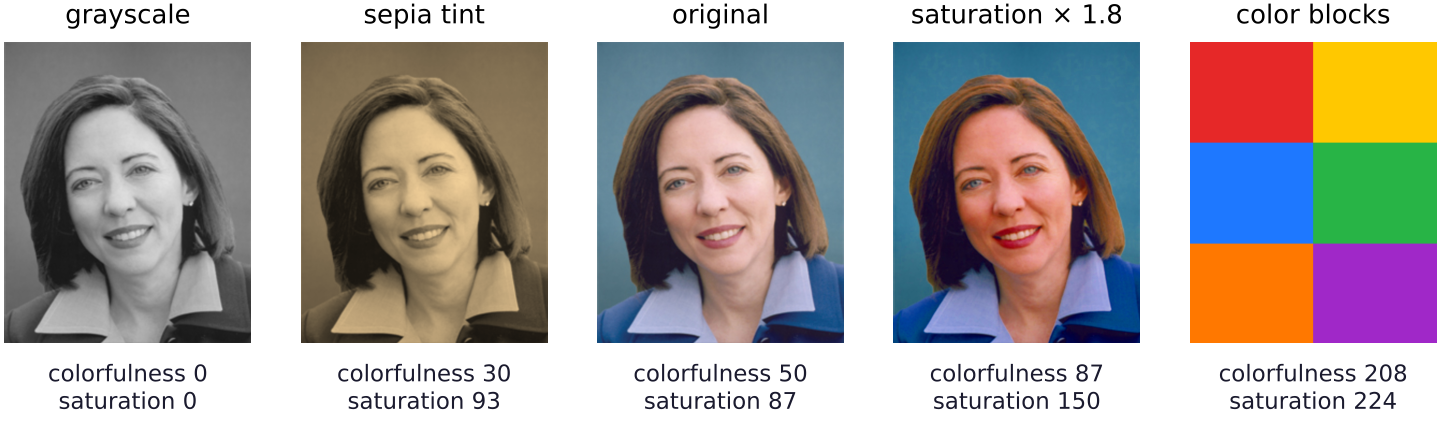
\includegraphics[width=0.74\textwidth]{figures/colorfulness_examples.png}

\raggedright
\muted{The sepia tint is \emph{more} saturated than the original but \emph{less} colorful: the
formula rewards variety, not a uniform tint.}
\end{frame}

% ─────────────────────────────────────────────────────────────────────────────
\begin{frame}{Which Colors? Palettes with k-Means}
\begin{columns}[c]
\begin{column}{0.55\textwidth}
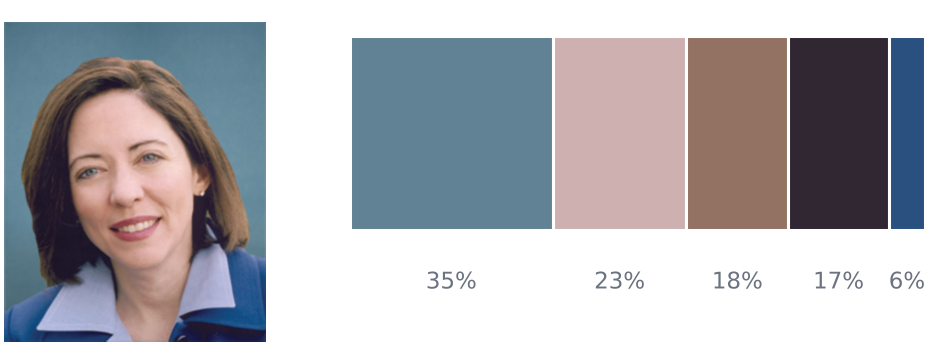
\includegraphics[width=\textwidth]{figures/palette.png}
\end{column}
\begin{column}{0.42\textwidth}
\begin{itemize}
\item Each pixel is a point in RGB space
\item \keyterm{k-means} finds $k$ cluster centers (the dominant colors) and the share of pixels
      closest to each
\item Cluster a downscaled copy: much faster, nearly the same result
\end{itemize}
\end{column}
\end{columns}

\vspace{0.2cm}
\begin{greenbox}
\textbf{$k$ is a choice.} With $k = 3$, distinct colors merge into averages that may appear nowhere
in the image; with $k = 8$, a logo or a mascot's eyes get their own cluster. Like the number of
topics in a topic model: report it and check that your results hold for other values.
\end{greenbox}
\credit{Official portrait of Sen.\ Maria Cantwell, public domain, via unitedstates/images.}
\end{frame}

% ─────────────────────────────────────────────────────────────────────────────
\begin{frame}{Complexity and Symmetry}
\begin{columns}[T]
\begin{column}{0.36\textwidth}
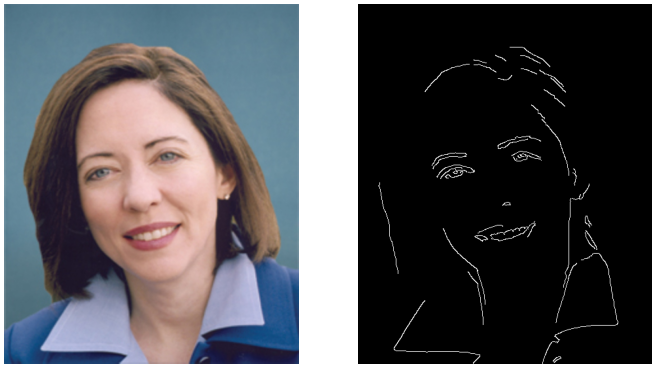
\includegraphics[width=\textwidth]{figures/edges.png}\\[2pt]
{\footnotesize Canny edges of the portrait}
\end{column}
\begin{column}{0.61\textwidth}
{\footnotesize
\begin{tabular}{@{}lp{4.4cm}r@{}}
\toprule
feature & what it captures & portrait \\
\midrule
edge density & share of pixels on an edge & 0.013 \\
bytes per pixel & JPEG size at quality 75: clutter & 0.084 \\
symmetry & 1 $-$ mean difference from the mirror image & 0.85 \\
\bottomrule
\end{tabular}}

\vspace{0.25cm}
\begin{warnbox}
\textbf{Correlated features are one finding, not two.} Edge density and bytes per pixel both
respond to detail; saturation and colorfulness both respond to strong colors. Check how your
features correlate before you count the evidence.
\end{warnbox}
\end{column}
\end{columns}
\end{frame}

% ─────────────────────────────────────────────────────────────────────────────
\begin{frame}{Faces with a Classic Detector}
\begin{columns}[T]
\begin{column}{0.38\textwidth}
\textbf{Viola--Jones (2001)}: slide windows of many sizes over the image; in each, test simple
light-and-dark patterns that faces share.

\vspace{0.15cm}
\centering
\begin{tikzpicture}[x=0.5cm, y=0.5cm]
\fill[darknavy] (0,0) rectangle (1,2); \draw[midgray] (0,0) rectangle (2,2);
\fill[darknavy] (3,1) rectangle (5,2); \draw[midgray] (3,0) rectangle (5,2);
\fill[darknavy] (6.66,0) rectangle (7.33,2); \draw[midgray] (6,0) rectangle (8,2);
\end{tikzpicture}\\[2pt]
{\footnotesize Haar-like features: sum of light minus sum of dark. Eyes are darker than cheeks.}

\raggedright
\vspace{0.15cm}
\muted{Fast and transparent, with well-known blind spots: faces in profile, small faces, hats,
masks.}
\end{column}
\begin{column}{0.59\textwidth}
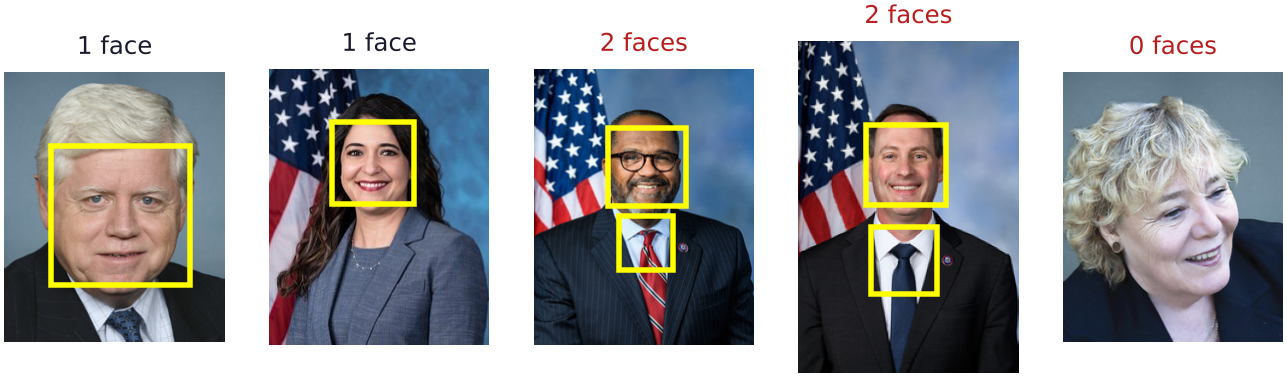
\includegraphics[width=\textwidth]{figures/faces_portraits.png}

\vspace{0.1cm}
\begin{greenbox}
\textbf{Validate where you know the answer.} Every portrait shows exactly one face. On 193
portraits the detector found exactly one in \textbf{94\%}; ten got extra ``faces'' (ties, flags),
one got none.
\end{greenbox}
\muted{\footnotesize On crowded protest photos it does much worse. Treat counts as a noisy lower
bound.}
\end{column}
\end{columns}
\end{frame}

% ─────────────────────────────────────────────────────────────────────────────
\begin{frame}{Reading Text with OCR}
\begin{columns}[T]
\begin{column}{0.45\textwidth}
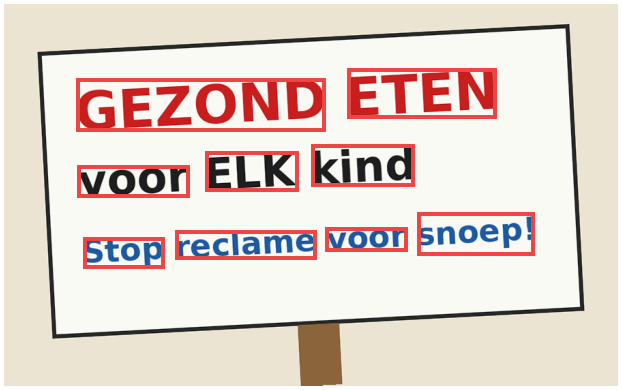
\includegraphics[width=\textwidth]{figures/ocr_sign.png}\\[2pt]
{\footnotesize A made-up protest sign, read by Tesseract (English and Dutch). Boxes: words kept.}
\end{column}
\begin{column}{0.52\textwidth}
\begin{tikzpicture}[
  b/.style={draw=wurgreen, fill=lightgreen, rounded corners=2pt, font=\footnotesize, align=center,
            inner sep=4pt, text width=4.6cm},
  arr/.style={-{Stealth[length=2mm]}, thick, color=midgray}]
\node[b] (a) {image $\rightarrow$ Tesseract};
\node[b, below=0.2cm of a] (b2) {every word with its box and a confidence (0--100)};
\node[b, below=0.2cm of b2] (c) {keep confidence $>$ 60 and $\geq$ 2 characters};
\node[b, below=0.2cm of c] (d) {\textbf{features:} number of words, share of the image covered by
text (here 0.18), the words themselves};
\draw[arr] (a) -- (b2); \draw[arr] (b2) -- (c); \draw[arr] (c) -- (d);
\end{tikzpicture}

\vspace{0.15cm}
\muted{\footnotesize Results depend on the language packs you load and on resolution: Tesseract's
documentation warns that accuracy drops when lowercase letters are under about 20 pixels tall.}
\end{column}
\end{columns}
\end{frame}

% ─────────────────────────────────────────────────────────────────────────────
\begin{frame}{Precise Is Not the Same as Valid}
\centering
\begin{tikzpicture}[
  c/.style={draw=darknavy, fill=darknavy, text=white, rounded corners=3pt, font=\footnotesize\bfseries,
            align=center, inner sep=5pt, text width=3.2cm},
  f/.style={draw=wurgreen, fill=lightgreen, rounded corners=3pt, font=\footnotesize, align=center,
            inner sep=5pt, text width=2.6cm},
  o/.style={draw=warnborder, fill=warnred, rounded corners=3pt, font=\scriptsize, align=center,
            inner sep=4pt, text width=2.4cm},
  arr/.style={-{Stealth[length=2mm]}, thick, color=midgray}]
\node[c] (con) {construct\\[2pt]\normalfont child-oriented design};
\node[f, right=2.2cm of con] (feat) {\textbf{colorfulness}\\score};
\node[o, right=1.4cm of feat, yshift=0.95cm] (o1) {background of the photo};
\node[o, below=0.15cm of o1] (o2) {lighting, white balance};
\node[o, below=0.15cm of o2] (o3) {camera, compression, cropping};
\draw[arr] (con) -- node[above=1pt, font=\scriptsize, color=midgray] {should drive} (feat);
\draw[arr, color=warnborder] (o1.west) -- (feat.east);
\draw[arr, color=warnborder] (o2.west) -- (feat.east);
\draw[arr, color=warnborder] (o3.west) -- (feat.east);
\end{tikzpicture}

\vspace{0.2cm}
\raggedright
\begin{columns}[T]
\begin{column}{0.48\textwidth}
\begin{graybox}
\textbf{Check against known truth}\\
like the portraits for the face detector: images where you know the right answer.
\end{graybox}
\end{column}
\begin{column}{0.48\textwidth}
\begin{graybox}
\textbf{Check against human judgment}\\
rate a sample yourself and correlate your ratings with the feature. Report it.
\end{graybox}
\end{column}
\end{columns}
\end{frame}

% ─────────────────────────────────────────────────────────────────────────────
\notebookslide{
\begin{itemize}
\setlength{\itemsep}{5pt}
\nbitem{\faSun}{Light and color for breakfast cereal packaging, by Nutri-Score}
\nbitem{\faPalette}{Palettes with k-means, and what $k$ does}
\nbitem{\faShapes}{Complexity, symmetry and which features measure the same thing}
\nbitem{\faUsers}{Faces: validated on portraits, then tried on protest crowds}
\nbitem{\faFont}{OCR on packaging in English and Dutch}
\nbitem{\faTable}{One feature table, the input for module 04}
\nbitem{\faRuler}{Your own ratings against the colorfulness score}
\end{itemize}

\vspace{0.35cm}
\muted{\footnotesize part1\_pixels/03\_handcrafted\_features/notebooks/03\_handcrafted\_features\_exercises.ipynb
· 7 exercises · CPU runtime}
}

\end{document}
